\section{Distributed Results}
\label{sec:distributed-result}

\begin{figure*}[tp]
    \centering
    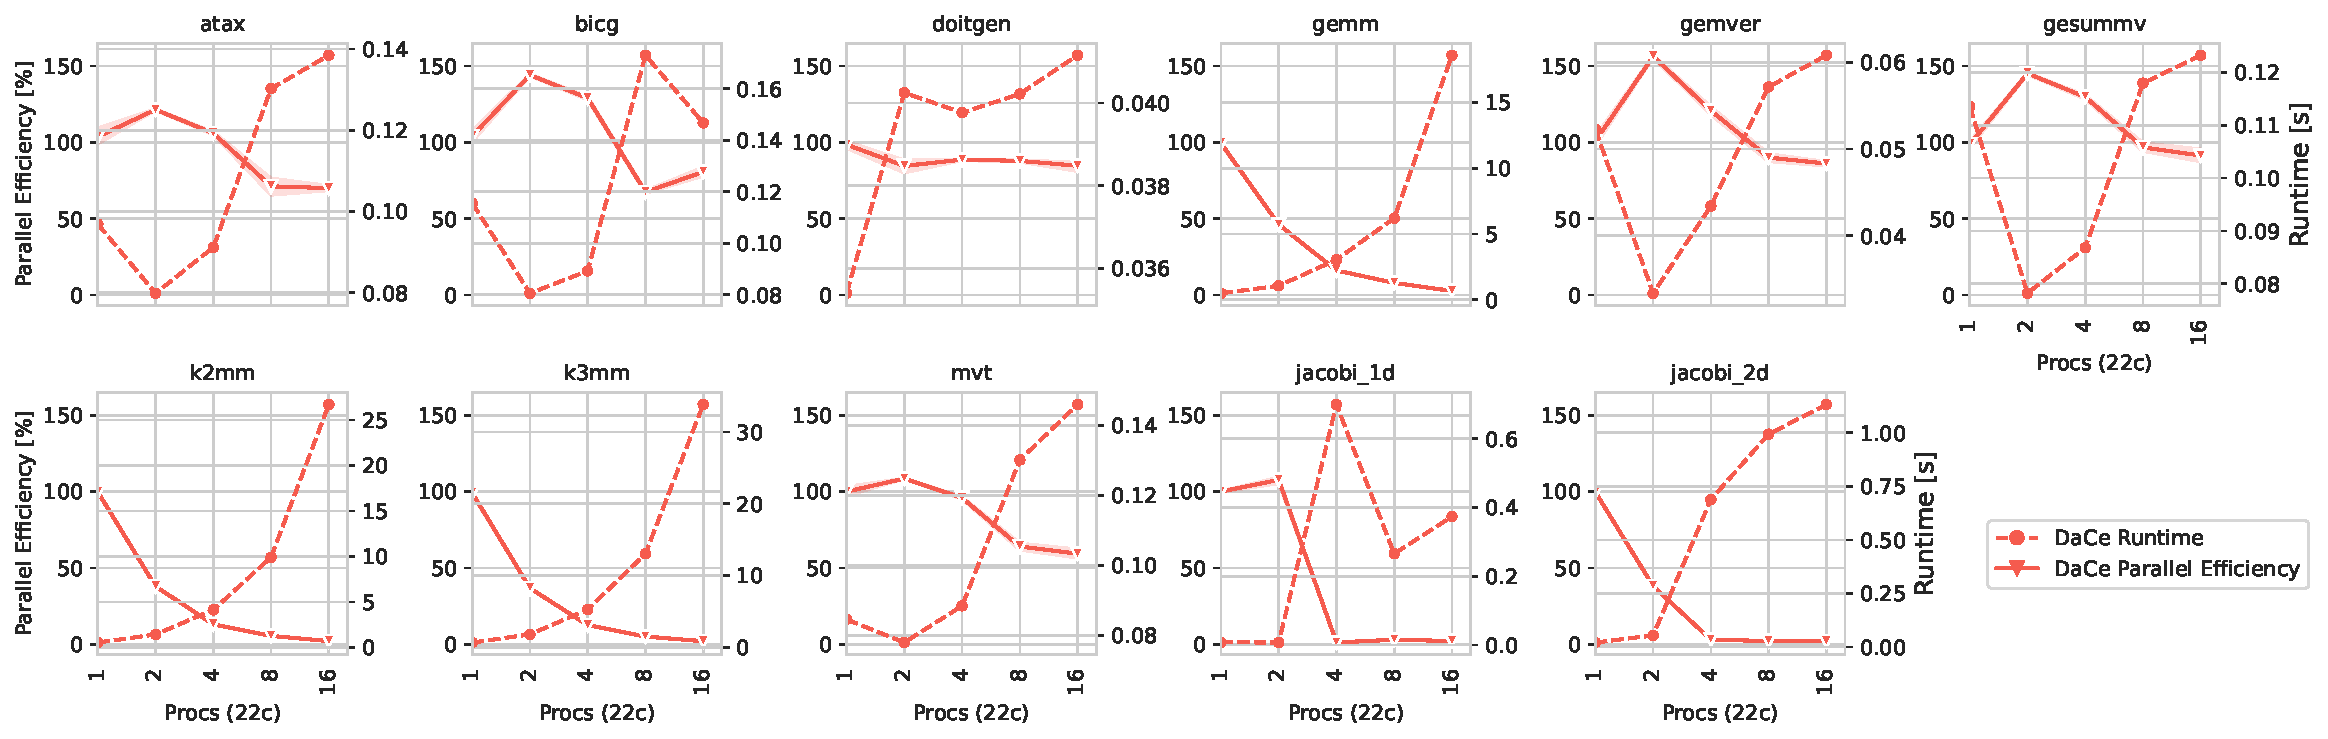
\includegraphics[width=.95\textwidth]{imgs/heatmap_distr.pdf}
    \caption{Distributed performance of DaCe on the Azure Cycle Cloud. The X-axis represents the number of processes, where each process is assigned to a single CPU socket (22 CPU cores). The dashed lines represent the runtime, while the solid lines represent the scaling efficiency.}
    \label{fig:heatmap_distr}
\end{figure*}

We evaluated the scalability of DaCe on our Azure cluster due to smaller scale of the physical cluster used in the SCC. We choose the "hb44rs" instance type, which is equipped with the Intel CPUs. Despite AMD CPUs' prowess in highly scalable workloads, DaCe relies on Intel MKL-ScaLAPACK for distributed computations, and some ScaLAPACK optimizations are tailored to Intel-specific structures, which resulted in reduced performance on AMD CPUs.

Figure~\ref{fig:heatmap_distr} illustrates our experimental results. Overall, our findings align with the original work. For instance, benchmarks that require minimal communication, such as \texttt{doitgen}, exhibit nearly perfect efficiency. However, we observed earlier degradation of parallel efficiency and significantly increased runtime variability in benchmarks with higher communication overhead. Notably, kernels like \texttt{atax}, \texttt{bicg}, \texttt{gemver}, \texttt{gesummv}, and \texttt{mvt}, responsible for matrix-vector products, exhibit optimal efficiency with 1 to 2 nodes but experience a rapid drop in efficiency when the scale exceeds 2 nodes.

This performance variation is influenced by both CPU and interconnect differences. The Piz Daint supercomputer used by the authors employs the 'Aries' interconnect from Cray with a dragonfly network topology, while Azure instances use a fat-tree style. Additionally, our Azure environment runs within virtual machines, and the communication libraries within these virtual machines aren't as optimized as those on dedicated supercomputers. These factors contribute to the increased runtime variation compared to the original paper~\cite{dace2021}.
% The parallel efficiency remains around 50\% for larger scales, as the communication library on the Azure cloud is not as optimized as dedicated supercomputers.


For the matrix-matrix product kernels, namely \texttt{gemm}, \texttt{k2mm}, and \texttt{k3mm}, the scalability is not ideal, which is an expected behavior of MKL-ScaLAPACK~\cite{matrixmatrix2019}. Such issues are also reported by the authors~\cite{dace2021}.

We reproduced the distributed experiments on our Azure cluster, providing insights into the scalability of DaCe. Despite observing efficiency degradation in certain scenarios, our results corroborate the original work and shed light on the behavior and limitations of MKL-ScaLAPACK in distributed computations.